% ============================================================================
%  第 1 章  概述
% ============================================================================
\chapter{概述}\label{ch:01}

\begin{flushright}
\small 第 1 讲；2021 年 1 月 19 日
\end{flushright}

\begin{keytakeaways}
本章给出全书的路线图。核心论点是：几何 Langlands 纲领应当被理解为一座连接数论与量子场论的桥梁，
更具体地说，是四维算术拓扑场论的两个对偶版本 $\mathcal{A}_G$ 与 $\mathcal{B}_{G^{\vee}}$ 之间的等价。
本章先回顾模形式/自守形式的经典图景：局部对称空间 $\Gamma\backslash G/K$ 上的 $L^2$ 谱理论、
Hecke 算子、周期与 Langlands 函子性；随后引入 Weil 的“罗塞塔石碑”，把数域、函数域与
Riemann 面放在同一张字典里，并说明为了容纳局部域与分歧数据，必须把字典升级为三维/四维的版本。
所使用的数学工具包括：约化群与算术格、局部对称空间、Hecke 代数、Galois 表示、局部系统与特征簇。
主要结论是式 \eqref{eq:1.34}：$\mathcal{A}_G\simeq\mathcal{B}_{G^{\vee}}$，它把自守侧的谱分解
与 Galois 侧的表示论组织成同一个 TFT 的两面。本章不含证明，只建立语言与直觉。
\end{keytakeaways}

\section{模形式/自守形式}
\begin{sectionkey}
本节把模形式与自守形式重新解释为局部对称空间上的谱问题：从 $\Gamma\backslash G/K$ 上的
$L^2$ 理论与双曲 Laplacian 出发，经 Eichler--Shimura 理论转入上同调；随后变动数域、
导子与 Hecke 算子，得到 Hilbert/Siegel 模形式、同余子群与 Hecke 本征值，最后以周期与
Langlands 函子性收束。核心图景是：自守形式是“基态”，Hecke 算子是守恒量，周期是测量。
\end{sectionkey}

\subsection{粗略想法}

模形式理论可以看成算术局部对称空间上的某种调和分析/量子力学。

局部对称空间的典型例子，是 $\mathrm{SL}_2(\Z)$ 作用在上半平面
$\mathbb{H}=\mathrm{SL}_2(\R)/\mathrm{SO}_2$ 上的基本域。换言之，我们考虑商空间
\begin{equation}\tag{1.1}\label{eq:1.1}
\mathcal{M}_{\mathrm{SL}_2\R}
  =\mathrm{SL}_2(\Z)\backslash\mathbb{H}
  =\mathrm{SL}_2(\Z)\backslash\mathrm{SL}_2(\R)/\mathrm{SO}_2 ,
\end{equation}
如图 \ref{fig:1-1} 所示。

对一般的约化代数群 $G$，可以考虑空间
\begin{equation}\tag{1.2}\label{eq:1.2}
\mathcal{M}_G=\Gamma\backslash G/K,
\end{equation}
其中 $\Gamma$ 是算术格，$K$ 是极大紧子群。眼下先限制在
\[
G=\mathrm{SL}_2(\R),\qquad
\Gamma=\mathrm{SL}_2(\Z),\qquad
K=\mathrm{SO}_2 .
\]
我们想在这个空间上做调和分析，也就是以有意义的方式分解其上的函数空间。在量子力学的情形，
我们主要关心 $L^2$ 函数：
\begin{equation}\tag{1.3}\label{eq:1.3}
L^2(\Gamma\backslash G/K),
\end{equation}
其上有双曲 Laplace 算子的作用。也就是说，我们要研究这个算子的谱理论。

同样的信息（或许以更易处理的形式）可以通过去掉 $K$ 得到。我们可以直接研究
\begin{equation}\tag{1.4}\label{eq:1.4}
\Gamma\backslash G=\mathrm{SL}_2(\Z)\backslash\mathrm{SL}_2(\R)
\end{equation}
上的 $L^2$ 函数；这是单位切丛，即前述空间上的一个圆丛。此时不再是研究 Laplacian，
而是利用齐性空间的结构研究整个 $\mathrm{SL}_2(\R)$ 的作用。

还可以把微分与多重微分纳入进来，即典范丛（的幂次）的截面：
\begin{equation}\tag{1.5}\label{eq:1.5}
\Gamma\bigl(\Gamma\backslash\mathbb{H},\,\omega^{k/2}\bigr).
\end{equation}

\begin{srcdef}{1}
$L^2(\Gamma\backslash G/K)$ 中的 $\Delta$-本征函数称为 \emph{Maass 形式}。
权为 $k$ 的模形式是 $\omega^{k/2}$ 的全纯截面。
\end{srcdef}

% [Tutor Note: 式 (1.5) 中的 $\omega^{k/2}$ 在 $k$ 为奇数时并不是通常意义下的线丛（需要 spin 结构，
%  或按自守因子的半整数权来理解）。作者在这里把“模形式 = 典范丛幂次的全纯截面”一笔带过，
%  严格处理需要引入覆盖群 $\mathrm{Mp}_2(\R)$ 或 metaplectic 结构；这是后续讨论半整数权模形式时的常见陷阱。]

\begin{srcrem}{1}
对拓扑学家而言，可能更愿意研究（拓扑）上同调（而不是微分形式），系数取某个局部系统
（即扭曲系数）。确实，模形式也可以来自 $\Gamma\backslash\mathbb{H}$ 的（扭曲）上同调，
这就是所谓的 \emph{Eichler--Shimura 理论}。

有人可能会担心，这样做离开了量子力学的世界；但转到上同调之后，我们做的其实是所谓的
\emph{拓扑量子力学}。相比“真正的”量子力学，本书会更关心前者。

这里的想法是：这个设定中没有动力学。我们只看基态，所以 Laplacian 为 $0$，只看调和的对象。
这确实与拓扑和上同调有关；而模形式正是某种基态。
\end{srcrem}

\begin{srcrem}{2}
如果取一般的 $G,K,\Gamma$，就得到更一般的\emph{自守形式}理论。
\end{srcrem}

\begin{figure}[htbp]
  \centering
  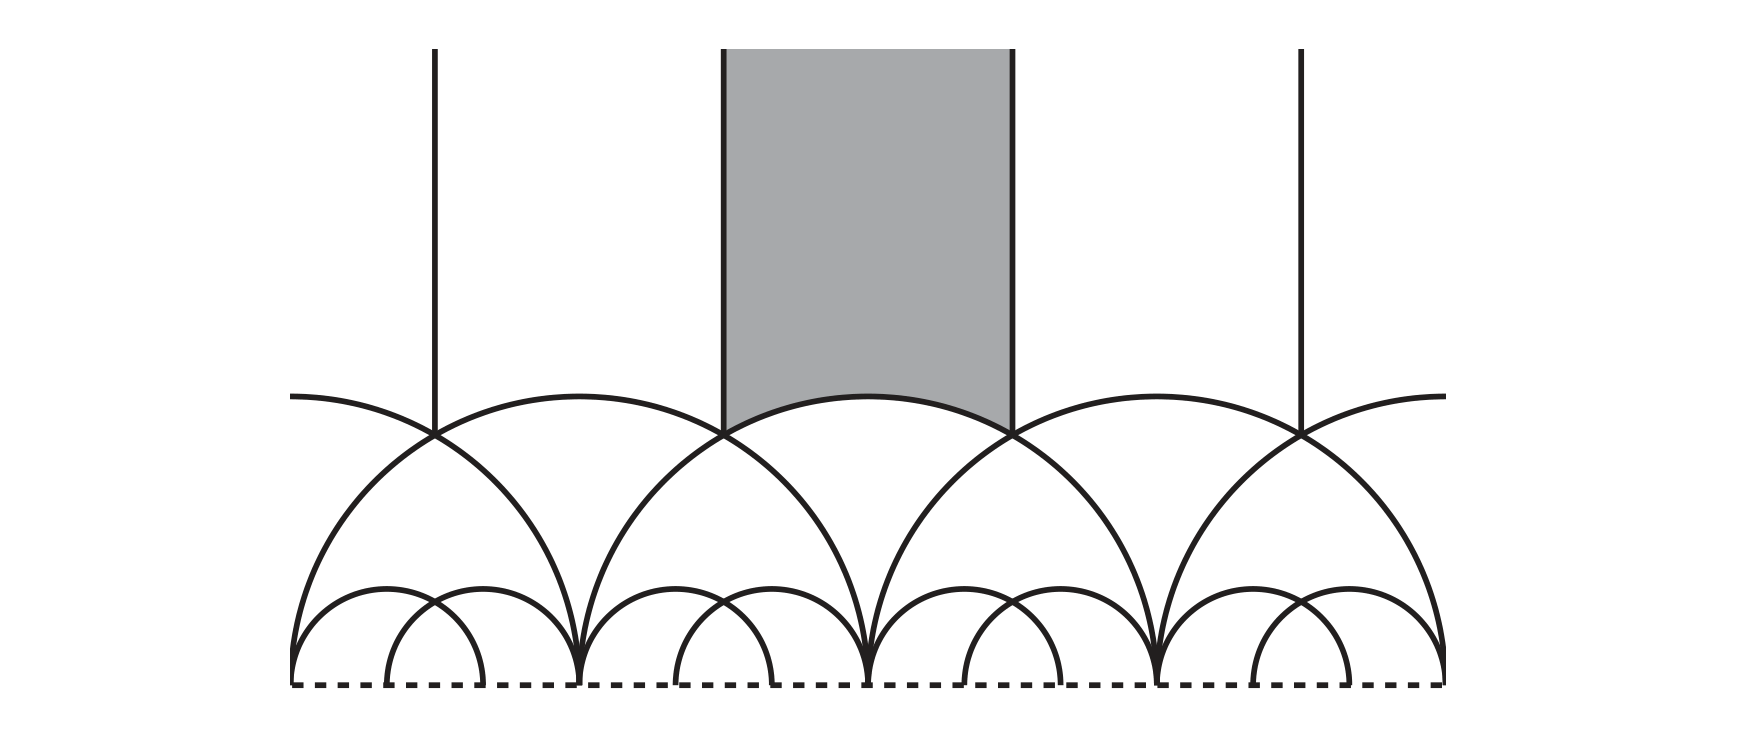
\includegraphics[width=0.52\textwidth]{figure1-1.png}
  \caption{$\mathrm{SL}_2(\Z)$ 作用在 $\mathbb{H}$ 上的基本域（灰色区域）。
    （原文 p.~10，Figure 1.1）}
  \label{fig:1-1}
\end{figure}

\begin{srcex}{1}
若取 $G=\mathrm{Sp}_{2n}(\R)$、$\Gamma=\mathrm{Sp}_{2n}(\Z)$、$K=\mathrm{SO}_n$，
就得到 \emph{Siegel 模形式}。
\end{srcex}

\subsection{结构}

把上述问题看成该局部对称空间上的量子力学，已有很长的历史。但数论中还存在着多得多的结构，
这些结构似乎并不出现在“粒子在该局部对称空间上运动”的量子力学里。

先把情形限制为 $G=\mathrm{SL}_2(\R)$。

\paragraph{数域}
理解
\begin{equation}\tag{1.6}\label{eq:1.6}
L^2\bigl(\mathrm{SL}_2(\Z)\backslash\mathrm{SL}_2(\R)/\mathrm{SO}_2\bigr)
\end{equation}
这一问题，对任意数域都有类比。可以把 $\Z$ 看成有理数域中的整数环：
\begin{equation}\tag{1.7}\label{eq:1.7}
\Z=\mathcal{O}_{\Q}.
\end{equation}
由此得到格 $\mathrm{SL}_2(\mathcal{O}_{\Q})$。这样写出来便可看出：可以把 $\Q$ 换成任意有限扩张 $F$，
于是 $\Z$ 变为整数环 $\mathcal{O}_F$：
\begin{equation}\tag{1.8}\label{eq:1.8}
\begin{aligned}
\Q &\rightsquigarrow F,\\
\Z &\rightsquigarrow \mathcal{O}_F .
\end{aligned}
\end{equation}

% [Tutor Note: 式 (1.8) 只是“换基域”的隐喻性图示，并不是说 $\mathcal{O}_F$ 等于 $\Z$ 作基变换。
%  正确的陈述是：$\mathcal{O}_F$ 是 $F$ 在 $\Q$ 上的整闭包；对 $F/\Q$ 有限，$\Spec\mathcal{O}_F$ 是 $\Spec\Z$ 上的有限平坦覆盖
%  （在分歧素点处退化）。把它读成“base change”会误导后续对分歧的几何理解。]

要点是：当把 $\Q$ 换成另一个数域 $F/\Q$ 时，空间 $\mathcal{M}_{G,\Q}$ 变成某个空间
$\mathcal{M}_{G,F}$。然后取 $L^2$ 或 $H^*$ 将其线性化。

\begin{srcex}{2}
这对所有约化代数群 $G$ 都成立；但取 $G=\mathrm{PSL}_2\R$，则
\begin{equation}\tag{1.9}\label{eq:1.9}
\mathcal{M}_{G,\Q}
  =\mathrm{PSL}_2\Z\backslash\mathrm{PSL}_2\R/\mathrm{SO}_2
\end{equation}
就是图 \ref{fig:1-1} 中的局部对称空间。若把 $\Q$ 换成任意数域 $F/\Q$，就得到
\begin{equation}\tag{1.10}\label{eq:1.10}
\mathcal{M}_{G,F}
  =\mathrm{PSL}_2(\mathcal{O}_F)\backslash
   \mathrm{PSL}_2(F\otimes_{\Q}\R)/K .
\end{equation}
注意
\begin{equation}\tag{1.11}\label{eq:1.11}
F\otimes_{\Q}\R\simeq \R^{\times r_1}\times \C^{\times r_2},
\end{equation}
其中 $r_1$ 是 $F$ 的实嵌入个数，$r_2$ 是复嵌入的共轭对个数。
\end{srcex}

% [Tutor Note: 式 (1.11) 中的记号 $\R^{\times r_1}$ 表示 $r_1$ 个 $\R$ 的直积，$\C^{\times r_2}$ 同理；
%  这里 $\times$ 是“笛卡尔积”而非群乘法。对 $F=\Q(\sqrt{d})$ 可直接验证：实二次域给出两个实嵌入，
%  虚二次域给出一个共轭对。后续计算 $\mathcal{M}_{G,F}$ 的维数/体积时，这个分解是第一道易错关口。]

\begin{srcex}{3}
令 $F=\Q\bigl(\sqrt{d}\bigr)$。若 $F$ 是实的（$d\ge 0$），则 $r_1=2$
（对应 $\pm\sqrt{d}$）、$r_2=0$，于是
\begin{equation}\tag{1.12}\label{eq:1.12}
\mathrm{PSL}_2\Bigl(\Q\bigl(\sqrt{d}\bigr)\otimes_{\Q}\R\Bigr)
  =\mathrm{PSL}_2\R\times\mathrm{PSL}_2\R .
\end{equation}
这引出所谓的 \emph{Hilbert 模形式}。

若 $F$ 是虚的（$d<0$），则 $r_1=0$、$r_2=1$，且
\begin{equation}\tag{1.13}\label{eq:1.13}
\mathrm{PSL}_2\Bigl(\Q\bigl(\sqrt{d}\bigr)\otimes_{\Q}\R\Bigr)
  =\mathrm{PSL}_2\C .
\end{equation}
此时极大紧子群是 $\mathrm{SO}_3\R$，商空间
\begin{equation}\tag{1.14}\label{eq:1.14}
\mathbb{H}^3=\mathrm{PSL}_2\C/\mathrm{SO}_3\R
\end{equation}
是双曲三维空间。接下来要用（左作用的）格作商，得到某个双曲流形，它是图 \ref{fig:1-1}
所示图景的三维版本。
\end{srcex}

\begin{srcrem}{3}
要点在于：变动数域后得到的实群并不那么有趣，只是一些 $\mathrm{PSL}_2$ 的拷贝；
但用来作商的格更强烈地依赖于数域，这才是有意思的部分。
\end{srcrem}

\paragraph{导子/分歧数据}
固定数域 $F=\Q$，可以变动“导子”或“分歧数据”。想法如下：局部对称空间 $\Gamma\backslash\mathbb{H}$
有一族覆盖空间 $\Gamma'\backslash\mathbb{H}$，其中 $\Gamma'$ 是 $\mathrm{SL}_2(\Z)$ 的某个同余子群。
于是可以把 $\Gamma$ 替换为 $\Gamma'$。

这里不一般地定义同余子群，但基本上有两类。对 $N\in\Z$，固定子群
\begin{equation}\tag{1.15}\label{eq:1.15}
\Gamma(N)=\left\{\begin{pmatrix}a&b\\ c&d\end{pmatrix}\equiv \mathrm{id}\pmod N\right\},
\end{equation}
\begin{equation}\tag{1.16}\label{eq:1.16}
\Gamma_0(N)=\left\{\begin{pmatrix}a&b\\ c&d\end{pmatrix}
  \equiv\begin{pmatrix}*&*\\ 0&*\end{pmatrix}\pmod N\right\}.
\end{equation}
想法是：从导子 $N$ 与格 $\Gamma$ 出发，然后在 $N$ 的因子处修改 $\Gamma$。注意即使在此设定中，
我们仍有 $\Gamma(N)$ 或 $\Gamma_0(N)$ 的选择。实际上这些变体构成的集合具有更多结构；
$p$ 处的局部数据与 $\mathrm{SL}_2(\Q_p)$ 的表示论有关。

\paragraph{Hecke 代数作用}
我们已经看到，Hilbert 空间依赖于群、数域以及某些分歧数据。

这个理论的一个非常重要的方面是：这个（函数）向量空间带有远为丰富的结构。这里存在巨大的
“退化”：Laplacian 的本征空间比人们预想的要大得多（不是一维的）。

这种退化由 \emph{Hecke 算子}理论给出。它说的是：Laplacian $\Delta$ 实际上属于一个巨大的
交换算子族，这些算子全都作用在 Laplacian 的本征空间上。对素数 $p$（$p$ 非分歧，即
$p\nmid N$），有 $p$ 处的 Hecke 算子 $T_p$。于是
\begin{equation}\tag{1.17}\label{eq:1.17}
\bigoplus_{p}\C[T_p]\ \circlearrowright\ L^2(\Gamma\backslash G/K).
\end{equation}
这是某种“量子可积系统”：如此多的算子与 Hamiltonian 交换，说明有许多守恒量。\footnote{%
这个例子在文献中常被当作量子混沌的例子（量子混沌是“可积性”的反面）。
混沌的一面与离散子群 $\Gamma$ 无关。更具体地说，这属于“算术量子混沌”的研究，
而后者更接近于可积系统的研究。}

\begin{figure}[htbp]
  \centering
  
\includegraphics[width=0.52\textwidth]{figure1-2.png}
  \caption{$\mathrm{SL}_2(\Z)$ 作用在 $\mathbb{H}$ 上的基本域（灰色）。
    可以这样定义“周期”：取一个模形式并在例如红线或蓝线上积分。
    （原文 p.~13，Figure 1.2）}
  \label{fig:1-2}
\end{figure}

\paragraph{周期/状态}
有一类特殊的测量可以作用于模形式，称为\emph{周期}（periods）。基本例子是沿直线
$i\R_+\subset\mathbb{H}$ 积分一个模形式，如图 \ref{fig:1-2}。Hecke 正是这样定义 $L$-函数的。

要点是：我们有一族性质非常好的测量/状态，于是可以通过这些周期来研究模形式。

\paragraph{Langlands 函子性}
还有一族略显神秘的算子，其作用对应于变动群 $G$。

\section{Langlands 纲领与 TFT}
\begin{sectionkey}
本节把自守侧的全部结构翻译成四维 TFT 的语言：数域对应三维流形，分歧数据对应余维 $2$
缺陷，Hecke 算子对应线缺陷，周期对应边界条件，函子性对应畴壁；而 $\mathcal{B}$-侧则把
$\pi_1$（或 Galois 群）的表示空间 $\Loc_{G^{\vee}}M$ 上的函数作为输出。由此得到全书主命题
$\mathcal{A}_G\simeq\mathcal{B}_{G^{\vee}}$，它是 Kapustin--Witten 电磁对偶的算术类比。
\end{sectionkey}

\subsection{概览}

我们已经看到，选定约化代数群 $G$ 与数域 $F/\Q$ 后，会得到一个局部对称空间
\begin{equation}\tag{1.18}\label{eq:1.18}
\mathcal{M}=\mathcal{M}_{G,F}
  =\text{“算术格”}\backslash\text{实群}/\text{极大紧子群}.
\end{equation}
它可以被看成 $G$-丛的某个空间
\begin{equation}\tag{1.19}\label{eq:1.19}
\mathcal{M}_{G,F}=\text{“}\Bun_G(\Spec\mathcal{O}_F)\text{”}.
\end{equation}
然后取 $L^2$ 或 $H^*$ 把这个空间线性化。

从自守形式理论出发，在 Hecke 代数作用下作谱分解。Langlands 纲领说：这个分解的各个碎片
对应于 Galois 表示。可以把自守形式理论想象成被送入一个棱镜，从另一侧出来的“颜色”就是
Galois 表示，如图 \ref{fig:1-3}。更具体地说，这些“颜色”是表示
\begin{equation}\tag{1.20}\label{eq:1.20}
\Gal\bigl(\overline{F}/F\bigr)\longrightarrow G^{\vee}_{\C}.
\end{equation}

\begin{figure}[htbp]
  \centering
  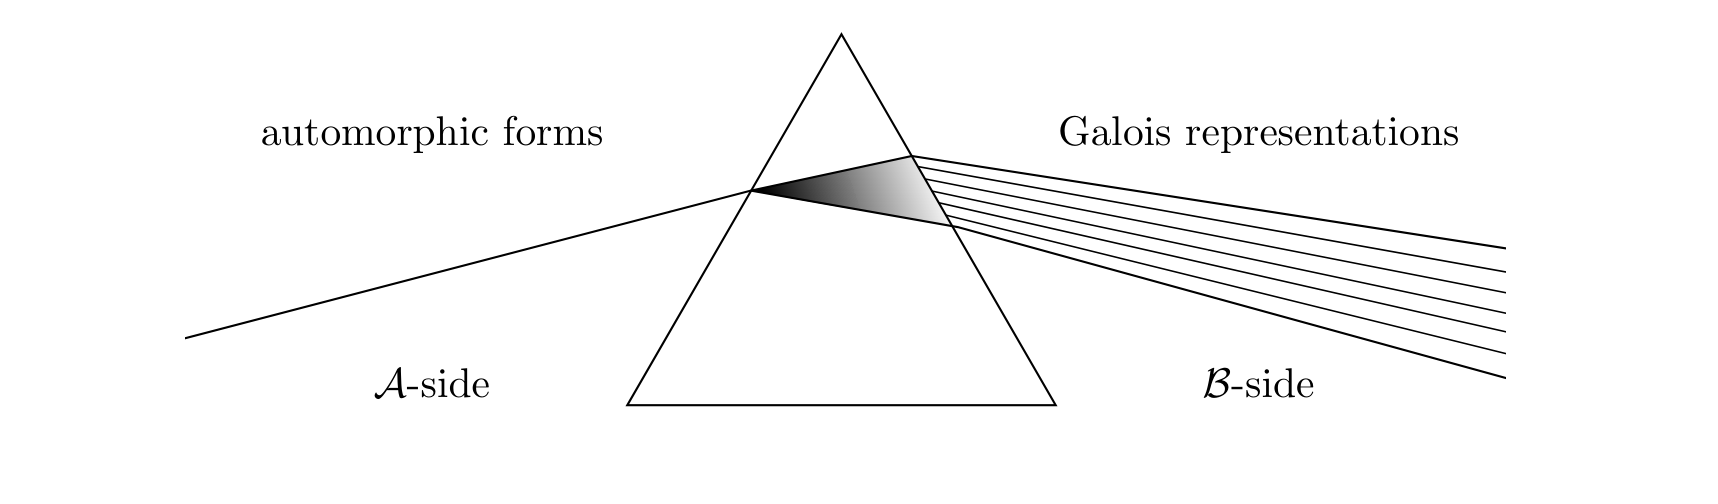
\includegraphics[width=0.55\textwidth]{figure1-3.png}
  \caption{正如光被棱镜分解，这种谱分解把自守形式（$\mathcal{A}$-侧）分解为
    数域的 Galois 表示（$\mathcal{B}$-侧）。（原文 p.~14，Figure 1.3）}
  \label{fig:1-3}
\end{figure}

% [Tutor Note: 式 (1.20) 中的 $G^{\vee}_{\C}$ 指 Langlands 对偶群的 $\C$-点，通常写作 $G^{\vee}(\C)$。
%  这里 $G$ 是 $\Q$ 上的约化群，$G^{\vee}$ 是其复对偶群；而 $\Gal(\overline{F}/F)$ 是绝对 Galois 群。
%  对 $G=\mathrm{GL}_n$，$G^{\vee}=\mathrm{GL}_n(\C)$，这正是通常的 $n$ 维 Galois 表示。对一般 $G$，
%  “$G^{\vee}$-值表示”需要把 Galois 表示与对偶群的中心/连通分量问题一起考虑。]

\begin{srcex}{4}
若 $G=\mathrm{GL}_2\R$，则 $G^{\vee}=\mathrm{GL}_2\C$。设 $E$ 是椭圆曲线，则
\begin{equation}\tag{1.21}\label{eq:1.21}
H^1(E/\Q)
\end{equation}
是 $\Gal(\overline{\Q}/\Q)$ 的二维表示。这正是这个设定中会出现的表示类型。
\end{srcex}

\begin{srcex}{5}
例 4 中的表示非常特殊，只适用于 $\mathrm{GL}_2$。若从 $\mathrm{GL}_3(\R)$ 出发，
相应的局部对称空间 $\mathrm{O}_3\backslash\mathrm{GL}_3\R/\mathrm{GL}_3\Z$
并不是复流形。
\end{srcex}

我们的目标是：把第 \ref{ch:01} 章第 1.1.2 节中的全部结构，与某个物理问题对应起来。
但普通的量子力学太简单了；在物理侧，我们将转而考虑量子场论。

\begin{quote}
\textbf{口号：} Langlands 纲领是四维（算术、拓扑）量子场论研究的一部分。
\end{quote}

具体想法是：Langlands 纲领是四维算术拓扑场论（TFT）之间的等价
\begin{equation}\tag{1.22}\label{eq:1.22}
\begin{array}{ccc}
\mathcal{A}_G & \simeq & \mathcal{B}_{G^{\vee}}\\[2pt]
\text{自守的（automorphic）} & & \text{谱的（spectral）}\\
\text{磁的（magnetic）} & & \text{电的（electric）}
\end{array}
\end{equation}
这两个理论分别称为 $\mathcal{A}$-侧与 $\mathcal{B}$-侧理论。

\begin{srcrem}{4}
这可以称为“四维镜像对称”。这里的 $\mathcal{A}$ 与 $\mathcal{B}$，与通常镜像对称中的
$\mathcal{A}/\mathcal{B}$ 是同一意义。
\end{srcrem}

% [Tutor Note: 式 (1.22) 的物理来源是 Kapustin–Witten 对 4d N=4 超对称 Yang–Mills 的
%  S-对偶作拓扑扭转；A-侧对应自守/磁侧，B-侧对应谱/电侧。它不是已证明的定理，
%  而是组织猜想的原则。这里作者用“等价”一词，读者应理解为“conjectural equivalence
%  of TFTs”；严格陈述需要指明边界条件、算子与范畴的层级。]

一个 $n$ 维 TFT 是这样一种对象：它对每个 $(n-1)$ 维流形指定一个量子力学问题
（或一个向量空间、链复形等）。所以四维 TFT 把三维流形送到某类向量空间。它对低维流形
指定更复杂的数据，对高维流形指定更简单的数据，如表 \ref{tab:1-1} 所示。

\begin{table}[htbp]
  \centering
  \caption{四维拓扑场论的输出。数是最容易理解的，但通常也最难产生（往往需要分析）。
    向量空间也相当简单，但三维流形很难；所以“最佳位置”大约在二维，因为曲面容易理解，
    而范畴也不算太复杂。（原文 p.~15，Table 1.1）}
  \label{tab:1-1}
  \begin{tabular}{c|l}
    \toprule
    Dimension & Output\\
    \midrule
    $4$ & $z\in\C$（很少能在代数上良定义，需要分析）\\
    $3$ & （微分分次）向量空间\\
    $2$ & （微分分次）范畴\\
    $1$ & $(\infty,2)$-范畴\\
    $0$ & $(\infty,3)$-范畴？（很少被理解）\\
    \bottomrule
  \end{tabular}
\end{table}

“拓扑”的意思是：我们扔掉动力学，只看基态。这类似于只看调和形式，而不是 Laplacian 的整个谱。
“算术”的意思是：我们遵循算术拓扑的范式。最终要在数域与三维流形之间建立类比；于是可以把
数域代入 TFT（代替真正的流形），得到一个向量空间，结果正是 $L^2(\mathcal{M}_{G,F})$
（或 $H^*(\mathcal{M}_{G,F})$）。

\subsection{算术拓扑}

\paragraph{Weil 的罗塞塔石碑}
在写给 Simone Weil 的一封信 \cite{Kri05} 中，André Weil 解释了一个漂亮的类比，
现在称为 \emph{Weil 罗塞塔石碑}。它在数域、函数域与 Riemann 面之间建立了三方类比。

一般想法如下。$\Spec\Z$ 是曲线的某种版本，其上的点 $\Spec\F_p$ 对应不同的素数。
$\Spec\Z_p$ 是点周围圆盘的版本，而 $\Spec\Q_p$ 是该点周围去心圆盘的版本。
这类似于代数曲线的通常图景。
\begin{center}
\begin{tabular}{lll}
  \toprule
  曲线 & $\Spec\F_q[t]$ & $\Spec\Z$\\
  点 & $\Spec\F_p$ & $\Spec\F_p$\\
  圆盘 & $\Spec\F_q[[t]]$ & $\Spec\Z_p$\\
  去心圆盘 & $\Spec\F_q((t))$ & $\Spec\Q_p$\\
  \bottomrule
\end{tabular}
\end{center}

% [Tutor Note: 原书此表“圆盘”一行印作 $\Spec\F_t[[t]]$（见 p.15），从上下文看应为
%  $\Spec\F_q[[t]]$：$q$ 是基域 $\F_q$ 的基数，$t$ 是形式参数。这属于原稿笔误，译文按数学上正确的
%  $\F_q[[t]]$ 处理；若读者对照原 PDF 会发现此差异，特此说明。]

一般地，设 $F/\Q$ 是数域，则可考虑 $\mathcal{O}_F$，而 $\Spec\mathcal{O}_F$ 的点对应
$\mathcal{O}_F$ 中的素数。数域与函数域之间的类比如下：从有限域上的光滑射影曲线
$C/\F_q$ 出发，$F$ 的类比是有理函数域 $\F_q(C)$，$\mathcal{O}_F$ 的类比是正则函数环
$\F_q[C]$，最后 $\Spec\mathcal{O}_F$ 的点对应 $C$ 的点。

现在可能想把 $C$ 换成 Riemann 面。设 $\Sigma/\C$ 是紧 Riemann 面，则 $\mathcal{O}_F$ 中的素数
（从而 $C$ 的点）对应 $\Sigma$ 的点。$\Sigma$ 上的亚纯有理函数域 $\C(\Sigma)$ 是 $F$ 的类比。
为了得到 $\mathcal{O}_F$ 的类比，必须从 $\Sigma$ 中去掉一些点（在紧曲线上得不到非平凡函数）。
要点是：数域带有一些“无穷远点”，所以其类比并不是紧 Riemann 面，而是带若干标记点的曲面。
于是 $\mathcal{O}_F$ 的类比由 $\Sigma$ 上在这些点之外正则的函数组成。

这总结在表 \ref{tab:1-2} 中。

\begin{table}[htbp]
  \centering
  \caption{Weil 罗塞塔石碑最初的形态；它在这三列之间建立类比。我们最终会细化这本字典。
    设 $F/\Q$ 是数域，$C/\F_q$ 是有限域上的光滑射影曲线，$\Sigma/\C$ 是紧 Riemann 面。
    $\F_q(C)$ 表示有理函数域，$\F_q[C]$ 表示正则函数环，$\C(\Sigma)$ 表示 $\Sigma$ 上的
    亚纯有理函数。（原文 p.~16，Table 1.2）}
  \label{tab:1-2}
  \begin{tabular}{lll}
    \toprule
    数域 & 函数域 & Riemann 面\\
    \midrule
    $F/\Q$ & $\F_q(C)$ & $\C(\Sigma)$\\
    $\mathcal{O}_F$ & $\F_q[C]$ & 在 $\Sigma$ 的标记点之外正则的函数\\
    $\Spec\mathcal{O}_F$ & $C$ 的点 & $x\in\Sigma$\\
    \bottomrule
  \end{tabular}
\end{table}

\paragraph{缺失的拼块}
现在采取这样的观点：这块罗塞塔石碑缺了一块，我们本应考虑三维流形而不是 Riemann 面。
想法是：$\Sigma/\C$ 真正对应的是 $C/\F_q$。这体现在如下方式中。为了研究点，我们研究映射：
\begin{equation}\tag{1.23}\label{eq:1.23}
\Spec\F_q\hookrightarrow C.
\end{equation}
但从平展拓扑的观点看，$\Spec\F_q$ 并不是真正的点，它更像一个圆，因为
\begin{equation}\tag{1.24}\label{eq:1.24}
\Gal\bigl(\overline{\F}_q/\F_q\bigr)
  =\widehat{\Z}=\pi_1^{\text{étale}}\bigl(\Spec\F_q\bigr),
\end{equation}
其中 $\widehat{\Z}$ 表示 profinite 完备化。因此最好把它想象成一个被修改过的圆，
其中 $\widehat{\Z}$ 由 Frobenius 生成。总有映射
\begin{equation}\tag{1.25}\label{eq:1.25}
\Spec\overline{\F}_q\longrightarrow\Spec\F_q,
\end{equation}
于是可以把曲线提升到 $\overline{\F}_q$。这对应于把这些圆“展开”，即替换为它们的万有覆盖。
于是出现一个 $\R$ 因子，它不参与拓扑/上同调。

于是我们意识到：$\F_q$ 上的曲线具有过多的内部结构，无法与 Riemann 面匹配。

\begin{srcrem}{5}
映射 $\Spec\F_{q^n}\to\Spec\F_q$ 类似于圆的通常 $n$ 重覆盖。
\end{srcrem}

为了修补罗塞塔石碑，我们把 Riemann 面 $\Sigma$ 替换为 $S^1$ 上的某个 $\Sigma$-丛。
具体地说，若给定 $\Sigma$ 与微分同胚 $\varphi$，可以构造映射环面
\begin{equation}\tag{1.26}\label{eq:1.26}
\Sigma\times I\big/\bigl((x,0)\sim(\varphi(x),1)\bigr).
\end{equation}
想法是：若从有限域上的曲线出发，微分同胚 $\varphi$ 就像 Frobenius。

类似地，$\Spec\mathcal{O}_F$ 看起来像一条曲线，其中每个“点”都携带一个圆。所以这同样是
某种三维流形。

\begin{srcrem}{6}
这些圆彼此之间并不“交谈”，因为它们都与不同素数处的 Frobenius 有关。所以它们不太像
乘积或纤维化，而更像带有叶状结构的三维流形。
\end{srcrem}

这与已有的算术拓扑理论相符，该理论有时被称为“纽结与素数”的类比。它始于 Mumford 写给
Mazur 的一封信，但可以归功于许多人，例如 Mazur \cite{Maz73}、Manin、Morishita \cite{Mor10}、
Kapranov \cite{Kap95} 与 Reznikov。Minhyong Kim 的近期工作 \cite{Kim15,CKK19} 起着核心作用。

\begin{srcrem}{7}
这本字典的许多方面已被明确写出，但不应过于直接地使用它。更确切地说，我们应把它理解为：
存在好几类“三维流形”——通常的三维流形、有限域上的函数域，以及数域。
\end{srcrem}

\begin{flushright}
\small 第 2 讲；2021 年 1 月 21 日
\end{flushright}

\paragraph{升级版的罗塞塔石碑}
要点是：我们把罗塞塔石碑中的三个对象都看成三维流形。特别地，把 $\Spec\mathcal{O}_F$
（例如 $\Spec\Z$）看成一个三维流形；于是对任意素数 $p$，有环路
$\Spec\F_p\to\Spec\mathcal{O}_F$，可以把它解释为该三维流形中的一个纽结。
设 $F_v$ 是 $F$ 在素点 $v$ 处的完备化（例如 $\Q_p$），则 $\Spec F_v$ 竟然是该纽结的
管状邻域的边界。要点是：若 $F_v$ 是非 Archimedes 局部域（例如 $\Q_p$ 或 $\F_p((t))$），
其“基本群”就是 Galois 群，并且有商
\begin{equation}\tag{1.27}\label{eq:1.27}
\Gal\bigl(\overline{F}_v/F_v\bigr)\twoheadrightarrow\Z_{\ell}\rtimes\widehat{\Z}.
\end{equation}
这个群称为 \emph{Baumslag--Solitar 群}。具体地，
\begin{equation}\tag{1.28}\label{eq:1.28}
\mathrm{BS}(1,p)=\bigl\{\sigma,u\ \bigm|\ \sigma u\sigma^{-1}=u^{p}\bigr\},
\end{equation}
其中把 $\sigma$ 看作 Frobenius，对应 $\widehat{\Z}$；$u$ 是 $\Z_{\ell}$ 的生成元。其核为
\begin{equation}\tag{1.29}\label{eq:1.29}
p\text{-群}\times\prod_{\ell'\neq\ell,p}\Z_{\ell'}
  \hookrightarrow \Gal\bigl(\overline{F}_v/F_v\bigr)
  \twoheadrightarrow\Z_{\ell}\rtimes\widehat{\Z}.
\end{equation}

% [Tutor Note: 式 (1.27)–(1.29) 描述的是局部域绝对 Galois 群的驯分歧商：
%  惯性群 $I_v$ 的驯部分同构于 $\prod_{\ell'\neq p}\Z_{\ell'}(1)$，而野惯性群是 pro-$p$ 群；
%  商 $\Z_{\ell}\rtimes\widehat{\Z}$ 中的 $\Z_{\ell}$ 来自 $\ell$-进循环（$\ell\neq p$），$\widehat{\Z}$ 由 Frobenius 生成。
%  原文在 (1.29) 前有一句残句 “This tells us that there is For p=1, ...”，
%  其中 “there is” 之后的文字被截断/错位；“p=1” 与 “p=-1” 也不是素数，
%  而是 Baumslag–Solitar 群的退化参数。译文按 BS(1,1)=Z²、BS(1,-1)=Klein 瓶的基本群处理，
%  并保留原文的表述方式。]

这说明：当 $p=1$ 时，这个群是 $\Z\times\Z=\pi_1(T^2)$；当 $p=-1$ 时，它是 Klein 瓶的
基本群。这提供了证据：$\Spec F_v$ 的平展基本群看起来像是环面基本群的某种依赖于 $p$ 的版本。
于是可以把 $\Spec F_v$ 看成一个二维流形（纤维化在 $S^1$ 上）。

经过这番讨论，我们可以给出升级版（多维）的罗塞塔石碑。在三维，我们有：
$\Spec\mathcal{O}_F$、$C/\F_q$，以及映射环面 $T_{\varphi}(\Sigma)$。前两者构成
\emph{整体算术}设定。在二维，首先有局部域，分两类：一类是有限扩张 $F_v/\Q_p$，
另一类是 $\F_q((t))$。这两者的 Spec 都是“二维”的，后者是某种去心圆盘 $D^*$。
它们构成\emph{局部算术}设定。代数闭域（正特征）上的曲线 $C/\overline{\F}_q$ 与
Riemann 面（$\C$ 上的射影曲线 $\Sigma$）也都是“二维”的，它们构成\emph{整体几何}设定。
我们唯一会考虑的四维流形是 $M^3\times I$ 或 $M^3\times S^1$ 的形式，其中 $M^3$ 是
算术或几何来源的三维对象。这些讨论总结在表 \ref{tab:1-3} 中。

\begin{table}[htbp]
  \centering
  \caption{各列对应 Weil 罗塞塔石碑的三个侧面，各行对应维数。我们考虑的四维对象
    只是三维对象与 $S^1$ 或 $I$ 的乘积。$M^3$ 是算术或几何来源的三维对象。
    三维对象是数域、函数域以及 Riemann 面的映射环面。$F$ 是数域，$\varphi$ 是 $\Sigma$
    的某个微分同胚，$T_{\varphi}$ 表示相应的映射环面构造。二维对象是局部域与曲线；
    $F_v$ 是 $\Q_p$ 的有限扩张。一维对象是两种版本的圆，零维对象是点。
    （原文 p.~18，Table 1.3；原表以图像保留）}
  \label{tab:1-3}
  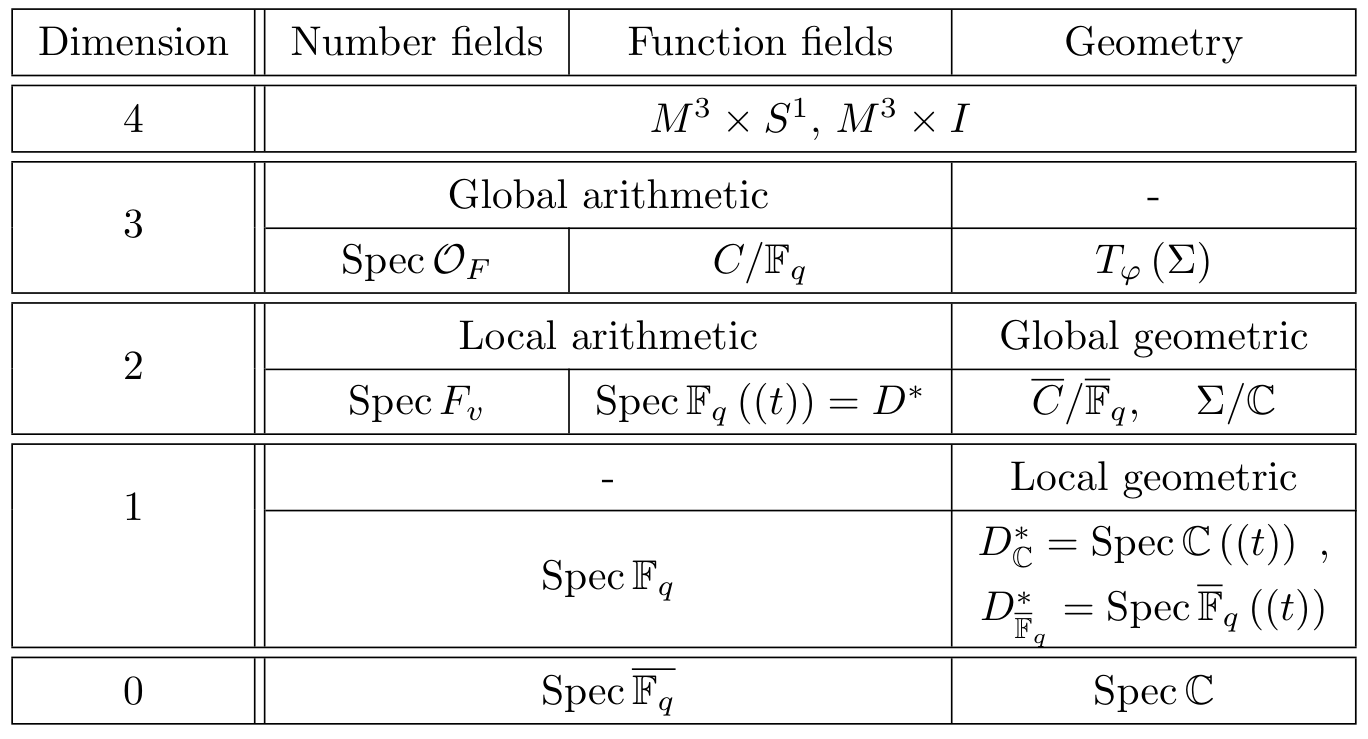
\includegraphics[width=0.82\textwidth]{table1-3.png}
\end{table}

\subsection{$\mathcal{A}$-侧}

$\mathcal{A}$-侧（或自守/磁侧）TFT $\mathcal{A}_G$ 是一台巨大的机器，能做的事很多，
如表 \ref{tab:1-1}。目前唯一能认出的东西是：它把三维流形 $M$ 送到某个向量空间
$\mathcal{A}_G(M)$。我们把 $\Spec\mathcal{O}_F$ 看成三维流形，而对应的赋值正是前面
一直在讨论的向量空间：
\begin{equation}\tag{1.30}\label{eq:1.30}
\mathcal{A}_G(\Spec\mathcal{O}_F)
  =L^2(\mathcal{M}_{G,F})\quad\text{或}\quad H^*(\mathcal{M}_{G,F}).
\end{equation}

\begin{srcrem}{8}
如式 (1.19) 所暗示的，注意 $\Gamma\backslash G/K$ 是所论三维流形上某个东西的模空间，
而不是三维流形本身。
\end{srcrem}

\subsection{结构（重奏）}

事实证明，第 1.1.2 节中自守形式理论的种种“铃铛与哨子”，与 TFT 的种种“铃铛与哨子”
完美地对齐了。

\paragraph{数域}
式 (1.30) 中的赋值形式化了如下想法：我们得到了一个由群与数域标记的向量空间
$L^2(\mathcal{M}_{G,F})$。

\paragraph{导子/分歧数据}
回想分歧数据是一串素数。它体现为三维流形中的一个链环（一族纽结），并允许奇点。
在物理中，它们表现为（余维 $2$ 的）\emph{缺陷}。于是我们先前看到的结构，
体现为该理论的缺陷。

\paragraph{Hecke 代数}
Hecke 算子对应场论中的线缺陷（余维 $3$）。物理上，这相当于沿时空中某个环路
“产生磁单极子”。

\paragraph{周期/状态}
它们对应边界条件，即余维 $1$ 的缺陷。

\paragraph{Langlands 函子性}
从 $G$ 过渡到 $H$，可以解释为穿过畴壁（同样是余维 $1$ 的缺陷）。

\subsection{$\mathcal{B}$-侧}

从数论的观点看，$\mathcal{B}$-侧（或谱侧）是困难的部分，因为数域的 Galois 群
（及其表示）非常难。也就是说，$\mathcal{B}$-侧是问题，而 $\mathcal{A}$-侧是答案。
但从几何的观点看恰好相反，因为 Riemann 面的基本群非常容易。
$\mathcal{B}$-侧研究的是 Galois 表示空间的代数几何。

% [Tutor Note: 原文此处印作 “The B-wide is about studying...”，其中 “B-wide” 显然是
%  “B-side” 的笔误（p.19）。译文按 B-side 处理。]

回想一下：给定三维流形（或数域 $F$），$\mathcal{A}$-侧关心算术局部对称空间
$\mathcal{M}_{G,F}$ 的拓扑。$\mathcal{M}_{G,F}$ 与 $F$ 的几何有关，所以 $\mathcal{A}$-侧
关心 $F$ 的几何的拓扑。

$\mathcal{B}$-侧关心 $F$ 的拓扑的代数。具体如下。对流形 $M$（任意维），可以构造
$\pi_1(M)$。于是 $M$ 上秩 $n$ 局部系统的集合为
\begin{equation}\tag{1.31}\label{eq:1.31}
\Loc_n M=\bigl\{\pi_1(M)\to\mathrm{GL}_n\C\bigr\}.
\end{equation}
局部系统看起来像秩 $n$ 的局部常值层（或带平坦联络的向量丛），有时也称为\emph{特征簇}
（character variety）。然后可以研究 $\C[\Loc_n M]$。

也可以用喜欢的复 Lie 群 $G$ 替换 $\mathrm{GL}_n$，得到
\begin{equation}\tag{1.32}\label{eq:1.32}
\Loc_{G^{\vee}}M=\bigl\{\pi_1(M)\to G^{\vee}\bigr\}.
\end{equation}
它只依赖于 $M$ 的拓扑。

若把数域看成三维流形，则 $\pi_1$ 是 Galois 群的替身，所以这是 Galois 群表示的空间。
TFT 把任意三维流形 $M^3$ 送到 $\Loc_{G^{\vee}}$ 上的函数：
\begin{equation}\tag{1.33}\label{eq:1.33}
\mathcal{B}_{G^{\vee}}\bigl(M^3\bigr)=\C\bigl[\Loc_{G^{\vee}}M\bigr].
\end{equation}

\begin{srcrem}{9}
这一侧写下来比 $\mathcal{A}$-侧容易得多；但若 $M$ 是数域，Galois 群可能非常难以理解。
其余那些“铃铛与哨子”在这里也都容易定义。
\end{srcrem}

\subsection{汇合}

在表 \ref{tab:1-3} 的所有设定中，我们要么作自守测量（附上 $\mathcal{M}_{G,F}$ 并研究其拓扑），
要么取 Galois 群（或 $\pi_1$），由它构造一个簇，再研究其上的代数函数。我们要解释的想法是：
Langlands 纲领是这两个庞大包裹之间的等价，但要对“Langlands 对偶群” $G$ 与 $G^{\vee}$ 而言：
\begin{equation}\tag{1.34}\label{eq:1.34}
\mathcal{A}_G\simeq\mathcal{B}_{G^{\vee}}.
\end{equation}

\begin{srcrem}{10}
在几何设定中已证明的内容比算术设定多，但即便对 Riemann 面的几何 Langlands，
仍是一个未解决的问题。
\end{srcrem}

这实际上是一种把一族猜想组织起来的猜想式方式。
